\documentclass[titlepage]{article}
\usepackage[utf8]{inputenc}
\usepackage{graphicx}
\usepackage{indentfirst}
\usepackage{dirtytalk}
\usepackage[margin=1in]{geometry}
\usepackage{latexsym, amsfonts, amssymb, amsthm, amsmath}

\usepackage{bera}% optional: just to have a nice mono-spaced font
\usepackage{listings}
\usepackage{xcolor}

\usepackage[english]{babel}
 
\setlength{\parindent}{4em}
\setlength{\parskip}{1em}
\renewcommand{\baselinestretch}{1.5}

\colorlet{punct}{red!60!black}
\definecolor{background}{HTML}{EEEEEE}
\definecolor{delim}{RGB}{20,105,176}
\colorlet{numb}{magenta!60!black}

\lstdefinelanguage{json}{
    basicstyle=\normalfont\ttfamily,
    numbers=left,
    numberstyle=\scriptsize,
    stepnumber=1,
    numbersep=8pt,
    showstringspaces=false,
    breaklines=true,
    frame=lines,
    backgroundcolor=\color{background},
    literate=
     *{0}{{{\color{numb}0}}}{1}
      {1}{{{\color{numb}1}}}{1}
      {2}{{{\color{numb}2}}}{1}
      {3}{{{\color{numb}3}}}{1}
      {4}{{{\color{numb}4}}}{1}
      {5}{{{\color{numb}5}}}{1}
      {6}{{{\color{numb}6}}}{1}
      {7}{{{\color{numb}7}}}{1}
      {8}{{{\color{numb}8}}}{1}
      {9}{{{\color{numb}9}}}{1}
      {:}{{{\color{punct}{:}}}}{1}
      {,}{{{\color{punct}{,}}}}{1}
      {\{}{{{\color{delim}{\{}}}}{1}
      {\}}{{{\color{delim}{\}}}}}{1}
      {[}{{{\color{delim}{[}}}}{1}
      {]}{{{\color{delim}{]}}}}{1},
}
\makeatletter
\setlength{\@fptop}{0pt}
\makeatother

\title{Communications Protocol Collaborative Spreadsheet}
\author{Richard Timpson \and
        Jabrail Ahmed \and 
        Tyler Brewster \and 
        Conner Grimes \and 
        Zack Muhlestein \and 
        Peter Forsling }
\date{\today}

\begin{document}

\maketitle

\tableofcontents

\section{Introduction}
The following document outlines a communications protocol for a client-server 
multi-user spreadsheet desktop application. The following protocol gives no 
information for either technologies used to implement the application on the 
client or server side, nor any details as to how the applications should be 
implemented. The protocol is split into two aspects, logging into the server 
and choosing a spreadsheet to edit, and editing a spreadsheet. All of the data 
transfer between client and server will happen using TCP and Sockets, and the 
data sent back and forth will be JSON.
    \subsection{Overview and Technologies}
    Put some more specific information here about the technologies 
    \subsection{Connection Overview}
    Give an overview about the connection 
    \subsection{Editing Overview}
    Give an overview about editing 
\section{Connection}
    \subsection{UML Diagram}
        \begin{figure}[p]
            \centering
            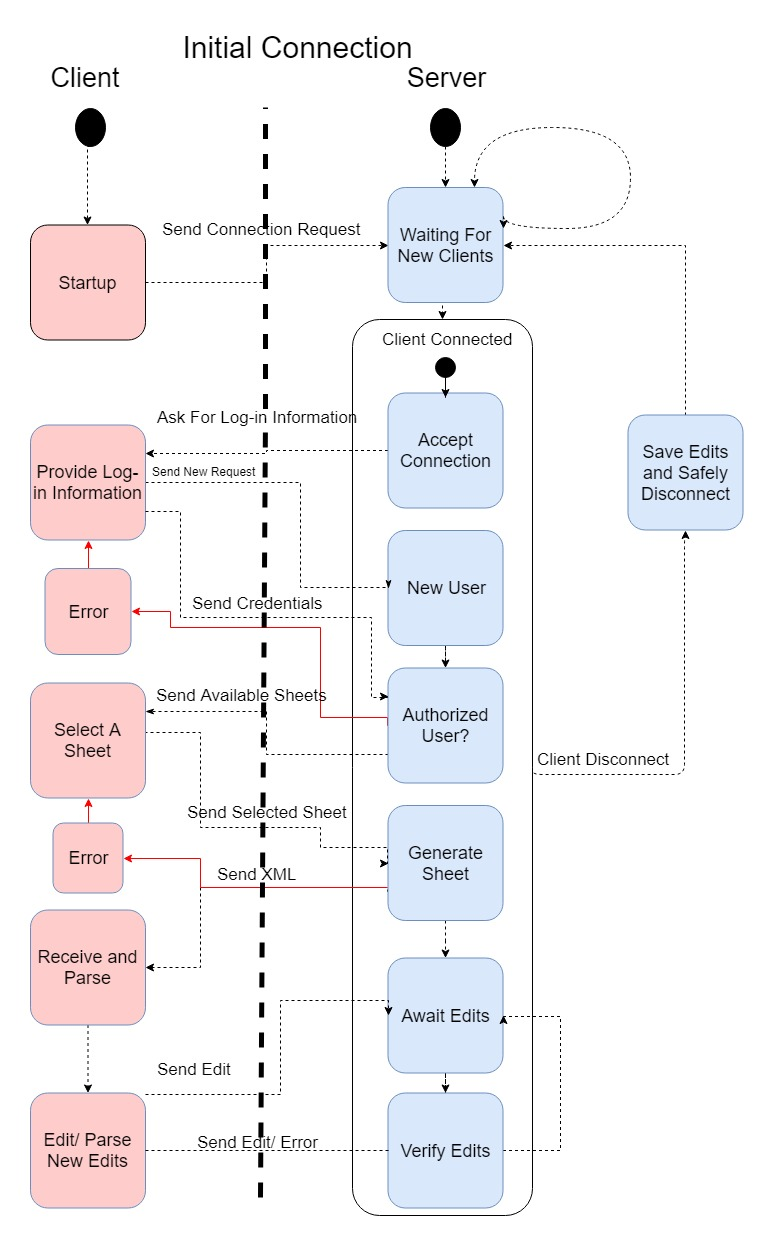
\includegraphics[width=.8\linewidth]{2-1}
            \caption{The UML diagram for the initial connection}
            \label{fig:connectionUML}
        \end{figure}
        Figure \ref{fig:connectionUML} shows what the initial connection of the client to the server 
            looks like as a process. The initial connection is broken up into two different
            phases; logging into the server and choosing a spreadsheet to edit. 
    \subsection{Socket Connection}
        Before a user logs into the server, there must be an initial connection from the client 
        to server so that they can begin communicating back and forth with each other. 
        The connection will be made using standard networking practices with a socket connection
        built over TCP/IP. On the initial start of the server, it should begin listening for socket
        connections at whatever IP address and port are sufficient. It is important that the client
        knows what specific IP address and port number to connect to. With this information, the 
        client should complete the socket connection with the server. If there are any errors with
        the connection, TCP should report them and both the client and server can handle the exceptions
        accordingly. If the connection is successful, the socket should stay connected to begin the
        transfer of data. 
        \begin{figure}[h]
            \centering
            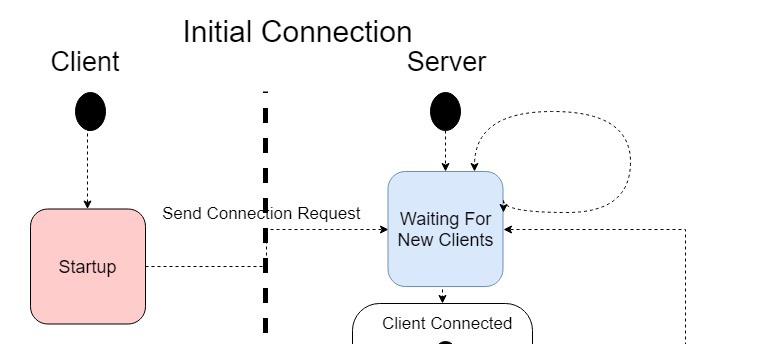
\includegraphics[width=1\linewidth]{2-2}
            \caption{The socket connection in \ref{fig:connectionUML}}
            \label{fig:socketUML}
        \end{figure}

    \subsection{Loggin In}
        Once the connection has been made, the server will expect the client, at some point in time,
        to send the information for either logging in, or creating a new user. This data will be sent
        as a JSON string terminated by a \say{n} character, as was discussed in the introduction 
        (need to make sure to talk about our data representation in the beginning of the document).
        Because the user can either log in or create a new user, there will be two different types of
        strings. For logging in, it will be formatted like so.

        \begin{lstlisting}[language=json,firstnumber=1]
        {
            "name": "the users name",
            "password": "the users password",
        }
        \end{lstlisting}
        If the client wants to create a new user, the string will formatted as such.
        \begin{lstlisting}[language=json,firstnumber=1]
        {
            "new_user": "true",
            "name": "the users name",
            "password": "the users password",
        }
        \end{lstlisting}
            
        It is the responsibility of the server to parse either string and perform the correct functionality
        based on that string, such as saving or checking the username and password. The server then needs
        to send a response back to the client, letting them know if the client successfully logged in or 
        created a new user. If for any reason the server could not validate the credentials, it should send
        an error message back to the client so that it knows that it failed to connect. The format for
        the success message is as follows...

        \begin{lstlisting}[language=json,firstnumber=1]
        {
            "success": "a boolean value that is true if successful, false if not",
            "message": "a message to the client letting them know what the error was if there was one, or if the user was successfully verified or created"
        }
        \end{lstlisting}

        If the client failed to log in, the server will expect another login message from the client,
        and will continue in this state until it receives valid login credentials. 

        \begin{figure}[h!]
            \centering
            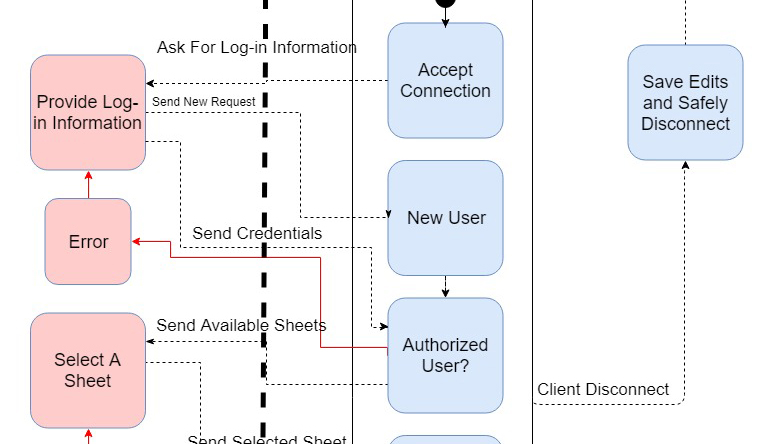
\includegraphics[width=1\linewidth]{2-3}
            \caption{Logging in in figure \ref{fig:connectionUML}}
            \label{fig:loginUML}
        \end{figure}

    \subsection{Picking a Spreadsheet}
        If the client did send valid login credentials, immediately after sending a success message,
        the server will send a JSON string containing an array of objects that contain information of
        the spreadsheets on that server that the user can access. The following string represents one
        valid spreadsheet object.

        \begin{lstlisting}[language=json,firstnumber=1]
        {
            "name": "the spreadsheets name",
            "id": "the spreadsheet id",
            "last_edit_date": "a date time  string in the format dd-mm-yyyy hh:mm:ss",
        }
        \end{lstlisting}

        The client then needs to send back to the server information about the spreadsheet it wants to select.
        As with logging in, the client can send two options for spreadsheet selection; either picking an existing
        spreadsheet or creating a new one. If the client wants to create a new spreadsheet, it need only send
        the name of the spreadsheet that it wants to create, like so. 
        \begin{lstlisting}[language=json,firstnumber=1]
        {
            "name": "name of the spreadsheet",
        }
        \end{lstlisting}
        If it wants to pick an existing spreadsheet, it should send the id of the spreadsheet that it would like.
        \begin{lstlisting}[language=json,firstnumber=1]
        {
            "name": "name of the spreadsheet",
        }
        \end{lstlisting}

        Again the server needs to send a message back to the client letting it know if it was successfully able to
        validate a spreadsheet for the client to edit. The JSON string should be the same as it is with logging in. 
        \begin{lstlisting}[language=json,firstnumber=1]
        {
            "success": "a boolean value that is true if successful, false if not",
            "message": "a message to the client letting them know what the error was if there was one, or if the user was successfully verified or created"
        }
        \end{lstlisting}

        Once the client has successfully chosen a spreadsheet to edit, the editing process will begin with the server
        sending all of the cells containing values as edits. 

        \begin{figure}[h!]
            \centering
            \includegraphics[width=.9\linewidth]{2-4}
            \caption{Logging in in figure \ref{fig:connectionUML}}
            \label{fig:loginUML}
        \end{figure}
            
\section{Editing}
\subsection{Overview}
    The basic process for editing a cell is as follows: the client enters a value into a cell and
    sends the cell’s information to the server. The server then checks to see if what the user
    has entered is a valid edit or not. After the server authorizes that the user has submitted a 
    valid edit, it sends that edit to all clients and records that edit. Figure \ref{fig:editUML} shows editing
    the spreadsheet as a process of communications between the client and the server.

    \begin{figure}[h!]
        \centering
        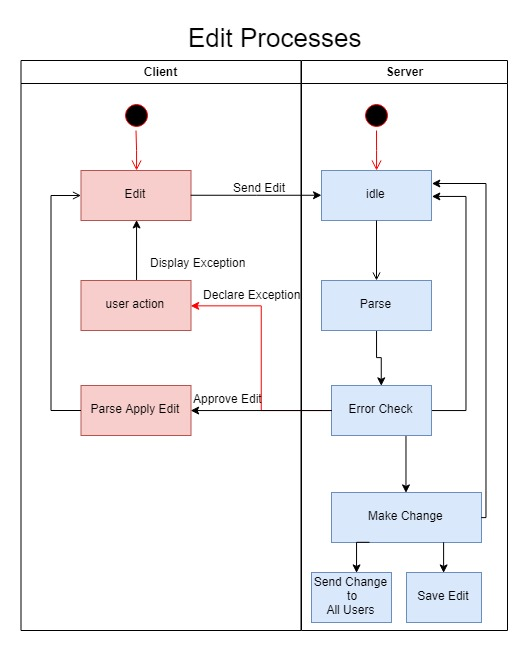
\includegraphics[width=.9\linewidth]{3-1}
        \caption{The editing diagram}
        \label{fig:editUML}
    \end{figure}
\subsection{Generating a saved spreadsheet}
    The server first sends the function code 0 followed by a JSON array containing all of the active users. Next, the server sends all of the non-empty cells as basic edits, following which it will send the locations of all other users for the client to display.  

    This is an example of the start up message from the server to the client:

    \begin{lstlisting}[language=json,firstnumber=1]
    0
    [
        {
            "cell": "two characters i.e a1",
            "users_active": ["userID1", "userID2", etc.],   
            "change": "",
            "value": "",     
        },
        {
            "cell": "two characters i.e a1",
            "users_active": ["userID1", "userID2", etc.],   
            "change": "",
            "value": "",     
        },
    ]
    \end{lstlisting}
\subsection{Basic Edit}
    After the client makes an edit locally it will send that edit to the server. The
    server will then validate the edit before sending that edit to all connected clients.
    If the edit is invalid it will say “formula error” or send it back as an exception.
    The server will also record this edit if it is not an exception. An example of a 
    basic edit message from the client to the server:
    \begin{lstlisting}[language=json,firstnumber=1]
    1
    {
        "user_name": "user's name",
        "cell": "A1",
        "change": "=5+5",
    }, 
    \end{lstlisting}
    And this is an example of a server to client message for basic edits:
    \begin{lstlisting}[language=json,firstnumber=1]
    2
    {
        "cell": "A1",
        "users_active": "",
        "change": "=5+5",
        "value": "10",
    }, 
    \end{lstlisting}
\subsection{Undo}
    After an undo option is called, the server will go back one edit chronologically. This will 
    NOT create a new edit. The latest edit will be deleted from record. This new change will
     then show up on the clients.
    \begin{itemize}
        \item When undo is called on an unedited spreadsheet, the server doesn’t need to do anything.
        \item A user should be able to call undo on a spreadsheet enough times to get it back to its original state (empty spreadsheet) from creation, regardless of the sheet being closed between creation and now. It is expected the server handles this functionality.
    \end{itemize}
    The following is an example of an undo request from client to the server:
    \begin{lstlisting}[language=json,firstnumber=1]
    2
    {
        "user_name": "users name",
        "cell": "A1",
        "change": ""// can also be seen as null,
    }, 
    \end{lstlisting}

\subsection{Revert}
    When the client calls for revert, the server will change the contents of the cell to its earlier
    contents. This new edit will be counted as a new edit. This change will then be evaluated and sent out
    as a normal edit.
    \begin{itemize}
        \item When revert is called on an unedited cell, the server doesn’t need to do anything.
        \item A user should be able to call revert on a cell enough times to get it back to its original
         state (empty cell) from creation, regardless of the sheet being closed between creation and now.
         It is expected the server handles this functionality.
    \end{itemize}
    When to people are editing a cell at the same time, the first edit sent will be the first edit parsed and the second edit will override the first edit.
    The following is an example of a revert request from the client to the server:
    \begin{lstlisting}[language=json,firstnumber=1]
    3
    {
        "user_name": "users name",
        "cell": "A1",
        "change": ""// can also be seen as null,
    }, 
    \end{lstlisting}
    
\subsection{Errors(Invalid Formulas)}
    When invalid formula error occurs we will give a notification in the cell block that says
     “Formula Error”. The following is an example message from the server to the clients:
     \begin{lstlisting}[language=json,firstnumber=1]
    3
    {
        "cell": "A1",
        "users_active": "",
        "change": "A1/+5"// can also be seen as null,
        "value": "Formula Error: Formatting",
    }, 
    \end{lstlisting}
\subsection{Exceptions(circular dependencies, divide by 0)}
    Exceptions do not count as edits and are not sent to all users. When divide by zero error
    occurs we give an exception to the user that entered the divide by zero exception. When
    a circular dependency occurs we must give a exception to the user that entered the circular 
    dependency to notify them of the exception. The following is an example message from the
    server to the client:

    \begin{lstlisting}[language=json,firstnumber=1]
    4
    {
        "cell": "A1",
        "users_active": "",
        "change": "Exception"// can also be seen as null,
        "value": "",
    }, 
    \end{lstlisting}

\subsection{Saving}
    When the client decides to save the current state of the spreadsheet the client should then 
    send the server a request to save so the server can authenticate that there are no exceptions 
    and then send the current state of the spreadsheet and save using a JSON objects. Also the 
    spreadsheet should be saved so that when the server unexpectedly crashes and make sure that 
    the last processed edit made by any user was saved.
    \begin{lstlisting}[language=json,firstnumber=1]
    5
    {
        "user_name": "users name",
        "cell": "", // can also be seen as null,
        "change": "" // can also be seen as null,
    }, 
    \end{lstlisting}

\subsection{Data Transfer}
    The following is the format of messages for our protocol. It follows the Json string format to
    simplify communication. No compression is expected for ease of communication between languages. 
    The following shows the expected format and fields with what the function number should be for 
    different expected results. 

    \subsubsection{Client to Server}
        \centering
        \begin{tabular}{| c | c | c |}
            \hline 
            Function Code & Course of Action & Value of Change\\ \hline
            0 & Editor Location Changed & 0 \\
            1 & Normal Cell Change & string \\
            2 & Undo Request & 0 \\
            3 & Revert Request & 0 \\
            4 & Client Changes Sheet & 0 \\
            5 & Save & 0 \\
            \hline            
        \end{tabular}
    \subsubsection{Server to Client}
        \begin{center}
            \begin{tabular}{| c | c | c | c | c |}
                \hline 
                Function Code & Course of Action & Value of users active & Value of change & Value of value\\ \hline
                0 & Start Setup & Array of current users & Null & Null \\
                2 & Edit Cell & Null  & String input & Calculated Value \\
                3 & Error & Null & String input & Formula Error \\
                4 & Exception & Null & "EXCEPTION" & 0 \\
                5 & Add/Remove Editor  & Array of current users & Null & Null \\
                \hline            
            \end{tabular}
        \end{center}
        \begin{center}
            \begin{tabular}{| c | c | c | c |}
                \hline 
                Function Code & Course of Action & Cell  & UserName \\ \hline
                1 & Change where someone is & Cell Number & User Number \\
                \hline            
            \end{tabular}    
        \end{center}
        
\section{Conclusion}
\end{document}
